While single-model prompting can achieve strong results, it often struggles with reliability, transparency, and adaptability in complex tasks. Recent work has therefore explored multi-agent systems, where large language models are organized as a group of cooperating agents with different roles. Instead of relying on one model to handle everything, tasks such as extraction, validation, and correction can be split into smaller parts, each performed by a specialized agent.

\begin{figure}[hbt!]
    \centering
    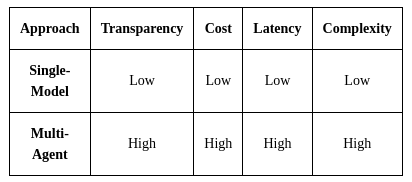
\includegraphics[width=0.5\linewidth]{images/single_vs_multi_model.png}
    \caption{Comparison of single-model and multi-agent approaches}
    \label{fig:placeholder}
\end{figure}

One of the best-known examples of this trend is HuggingGPT, introduced by Shen et al.\ \cite{shen2023hugginggpt}. In this framework, an LLM acts as a controller that delegates subtasks to external models hosted on the Hugging Face platform. The controller coordinates the results and integrates them into a final response. Liang et al.\ \cite{liang2023taskmatrix} proposed a similar system, TaskMatrix.AI, which connects LLMs with thousands of external APIs so that each subtask can be handled by the tool best suited for it. These studies show how LLMs can work as managers that coordinate specialized modules, rather than attempting to solve every step by themselves.

Other work has focused on applying multi-agent ideas directly to document and information extraction. Park et al.\ \cite{park2023generative} describe generative agents that cooperate to process documents: one agent extracts candidate entities, while another validates or reformats them according to schema constraints. This separation of roles reduces the cognitive load on any single model and makes the pipeline easier to debug, since errors can be traced back to a specific agent. Du et al.\ \cite{du2023improving} investigate multi-agent dialogue, where different agents simulate roles such as information seeker, verifier, and summarizer, in order to improve factual consistency. These ideas can be transferred to template filling, where one agent extracts fields, another checks them, and a third refines or corrects them.

Consensus-based multi-agent systems add another layer of reliability. Wu et al.\ \cite{wu2023autoagents} introduced AutoAgents, an open-source framework where multiple agents generate alternative outputs which are then compared, aggregated, or voted on. This ensemble-style approach reduces variance and improves robustness by leveraging diversity across agents. It mirrors classical redundancy methods but benefits from the contextual reasoning abilities of LLMs, making it especially useful in noisy or ambiguous input scenarios.

Despite their advantages, multi-agent systems face important challenges. They require more coordination and introduce overhead, since communication between agents can be costly and errors in one stage can still propagate. Designing reliable interfaces between agents is crucial, otherwise misalignments may cause cascading errors. In addition, evaluation of coordination quality is still underdeveloped; most benchmarks focus on the final output rather than the collaboration process itself. Finally, multi-agent pipelines often have longer latency and higher costs compared to single-model approaches.

In the context of this thesis, multi-agent systems are highly relevant because they address three requirements identified earlier: transparency, user correction, and adaptability. By splitting tasks into separate roles, they allow errors to be traced to specific stages (supporting transparency), corrections to be integrated incrementally, and domain knowledge to be embedded in specialized agents. At the same time, their higher cost and coordination complexity highlight trade-offs compared to simpler single-model systems. These trade-offs motivate the comparative evaluation carried out in this thesis, where multi-agent strategies are tested alongside monolithic and hybrid approaches.
